% =====================================================================
%  A Controlled Study of Fine-Tuning DINOv2 for Landmark Image Retrieval
%  Springer LNCS format (llncs.cls + splncs04.bst)
%  Compile:  pdflatex main && bibtex main && pdflatex main && pdflatex main
%  (Overleaf: upload the zip, compiler = pdfLaTeX)
% =====================================================================
\documentclass[runningheads]{llncs}

\usepackage[T1]{fontenc}
\usepackage{lmodern}
\usepackage{graphicx}
\usepackage{amsmath,amssymb}
\usepackage{booktabs}
\usepackage{multirow}
\usepackage{adjustbox}
\usepackage{xcolor}
\usepackage{tikz}
\usetikzlibrary{arrows.meta,positioning,fit,calc,shapes.geometric,backgrounds}
\usepackage[hidelinks]{hyperref}
\usepackage{url}

\newcommand{\roxf}{$\mathcal{R}$Oxford5k}
\newcommand{\rpar}{$\mathcal{R}$Paris6k}
\newcommand{\roxs}{$\mathcal{R}$Oxf}
\newcommand{\rpas}{$\mathcal{R}$Par}
\newcommand{\aqe}{$\alpha$QE}
\newcommand{\best}[1]{\textbf{#1}}

\definecolor{cfrozen}{HTML}{DCE6F2}
\definecolor{ctrain}{HTML}{F8D5BF}
\definecolor{chead}{HTML}{DDEFD9}
\definecolor{cpost}{HTML}{EFE3F6}
\definecolor{cgray}{HTML}{8A8A8A}

\emergencystretch=1.5em
\begin{document}

\title{A Controlled Study of Fine-Tuning DINOv2 for Landmark Image Retrieval}
\titlerunning{Fine-Tuning DINOv2 for Landmark Retrieval}

\author{Nguyen~Ngoc~Thanh~Nhan \and Tran~Long~Vu \and Nguyen~Hoang~Anh~Kiet \and Nguyen~Hai~Nguyen \and Nguyen~Hong~Quan \and Bui~Cao~Vu}
\authorrunning{N.~N.~T. Nhan et al.}
\institute{FPT University, Da Nang, Vietnam\\
\email{thanhnhan73.work@gmail.com, vutran.03092006@gmail.com,}\\
\email{kiet.nguyen20067@gmail.com, hainguyenzzz2201@gmail.com,}\\
\email{hongquannguyen2k6@gmail.com, vubc@fe.edu.vn}}

\maketitle

% ---------------------------------------------------------------------
\begin{abstract}
Content-based image retrieval (CBIR) at the instance level asks for every
database image that shows the \emph{same} object as the query, under strong
changes of viewpoint, scale, illumination and occlusion. Generalized-mean
(GeM) pooling over fine-tuned CNN activations, trained without human
annotation on structure-from-motion data, has been a standard global-descriptor
baseline for this task since 2018. In this paper we revisit the GeM pipeline
with a modern self-supervised Vision Transformer backbone (DINOv2 ViT-B/14)
and improve it through a strictly controlled, one-factor-at-a-time protocol in
which every new version changes exactly one design choice with respect to the
best previous version and states its motivation in advance. Starting from a
faithful rebuild of the GeM training recipe (contrastive loss, hard-negative
mining on retrieval-SfM-120k, learned whitening), we study the descriptor head
(GeM over patch tokens vs.\ the class token), the depth of partial
fine-tuning, the learning rate, and $\alpha$-weighted query expansion, and
we select versions on the retrieval-SfM-120k validation split rather than on
the test benchmarks. On the Revisited Oxford and Paris benchmarks, training on
the class token instead of GeM-pooled patch tokens is the single largest gain
(+7.8/+8.7 mAP on \roxf{} Medium/Hard over the GeM descriptor of the same
backbone), while fine-tuning more blocks or lowering the learning rate gives
equivalent models at about 72 mAP. Evaluated under exactly the same protocol,
the fine-tuned class token improves over the frozen DINOv2 backbone by
+1.9/+2.9 mAP on \roxf{} (72.0/52.8 vs.\ 70.1/49.8) and by +1.2/+1.1 on
\rpar{}; with \aqe{} on both sides the final global-only model reaches
74.1/54.6 on \roxf{} and 90.2/77.7 on \rpar{}, against 72.2/51.9 and 89.1/76.6
for the frozen backbone. Additional evaluation-only checks show that removing
the ReLU from GeM does not close the gap to the class token, and that
multi-scale inference hurts the class token only when it adds down-scaled
inputs. The whole study runs on a single free-tier T4 GPU; code and logs are
released.

\keywords{Content-based image retrieval \and Instance-level retrieval \and
Landmark retrieval \and GeM pooling \and Vision Transformer \and DINOv2 \and
Query expansion}
\end{abstract}

% =====================================================================
\section{Introduction}
\label{sec:intro}

Content-based image retrieval (CBIR) ranks the images of a collection by their
visual similarity to a query image, without relying on text or tags
\cite{smeulders2000cbir,srivastava2023cbir}. Its most demanding variant is
\emph{instance-level} retrieval, where a result is relevant only if it depicts
the very same object or place as the query, for example a particular
building photographed from a different side, at night, or partly hidden by
trees \cite{zheng2018sift,chen2023instance}. Landmark retrieval is the
canonical benchmark for this setting, and the Revisited Oxford and Paris
datasets (\roxf{}, \rpar) \cite{radenovic2018revisiting}, with their Medium
and Hard protocols, are the standard way to measure progress.

Over two decades the field moved from bag-of-visual-words on local SIFT
features \cite{sivic2003video,lowe2004sift,philbin2007oxford} to compact global
descriptors produced by convolutional networks
\cite{razavian2014cnn,babenko2014neural,babenko2015spoc,tolias2016rmac,gordo2017endtoend}.
Among the latter, the method of Radenovi{\'c} \emph{et al.}
\cite{radenovic2019gem} became a reference point: a CNN is fine-tuned with a
contrastive loss on image pairs mined automatically from 3D
structure-from-motion (SfM) models, its last feature map is aggregated by
\emph{generalized-mean} (GeM) pooling with a learnable exponent, and a
discriminative whitening is learned from the same SfM pairs. The recipe needs
no manual labels, produces a single vector per image, and is still used as the
global stage of state-of-the-art systems
\cite{cao2020delg,lee2022cvnet,shao2023superglobal}.

Since then, the backbone landscape has changed. Vision Transformers (ViTs)
\cite{dosovitskiy2021vit} trained with large-scale self-supervision, most
notably DINO \cite{caron2021dino} and DINOv2 \cite{oquab2024dinov2}, produce
features that already rival supervised retrieval models without any
fine-tuning. This raises a natural, practical question that this paper
answers experimentally: \emph{what happens when the well-understood GeM
training recipe is applied to a modern self-supervised ViT, and which parts of
the recipe still matter?}

Rather than proposing a new architecture, we follow a disciplined engineering
protocol. We first rebuild the GeM pipeline with only the backbone swapped
(ResNet-101 $\rightarrow$ DINOv2 ViT-B/14), which we call B0. Each subsequent
version B1, B2, \dots{} changes \emph{exactly one} factor with respect to the
best version so far, and the reason for the change (prior result, theory and
literature) is written down before the experiment is run. A version that does
not improve on the validation split is not used as a base, and the next one
branches from the previous best.

Our contributions are:
\begin{itemize}
\item A faithful, self-contained re-implementation of the GeM training and
evaluation pipeline (SfM tuples, hard-negative mining, contrastive loss,
learned whitening, revisited evaluation protocol) on top of DINOv2, runnable on
a single free-tier GPU.
\item A controlled one-factor-at-a-time study (B0--B4) of descriptor head,
fine-tuning depth, learning rate and query expansion, with model and \aqe{}
selection on a held-out validation split, a frozen-backbone baseline run under
the same protocol, and every intermediate number reported, including the
negative results.
\item The empirical finding that for a self-supervised ViT the class token is a
much better trainable global descriptor than GeM over patch tokens
(+7.8 mAP on \roxf{} Medium) and that this gap is not caused by the ReLU in
GeM; that multi-scale averaging with down-scaled inputs, which helps CNN
descriptors, \emph{hurts} the class token, while up-scaling does not; and that
further fine-tuning capacity saturates at about 72 mAP.
\item A global-only model reaching 74.1/54.6 mAP on \roxf{} and 90.2/77.7 on
\rpar{} (Medium/Hard), +1.9/+2.8 and +1.1/+1.1 above the frozen DINOv2
ViT-B/14 backbone with the same \aqe{} and evaluation code.
\end{itemize}

The rest of the paper is organized as follows. Section~\ref{sec:related}
reviews related work. Section~\ref{sec:method} describes the baseline, our
rebuild and the versioning protocol. Section~\ref{sec:setup} gives the
experimental setup, Section~\ref{sec:results} the results, and
Section~\ref{sec:discussion} discusses findings and limitations before
Section~\ref{sec:conclusion} concludes.

% =====================================================================
\section{Related Work}
\label{sec:related}

\paragraph{From local features to global CNN descriptors.}
Classical instance retrieval quantized local SIFT descriptors
\cite{lowe2004sift} into visual words and ranked images with inverted files
\cite{sivic2003video}, refined by spatial verification
\cite{philbin2007oxford,philbin2008paris} and aggregated encodings such as VLAD
\cite{jegou2010vlad}. Razavian \emph{et al.} \cite{razavian2014cnn} and
Babenko \emph{et al.} \cite{babenko2014neural} showed that activations of
ImageNet-trained CNNs are strong off-the-shelf descriptors. Pooling the last
convolutional map then became the dominant design: sum pooling (SPoC)
\cite{babenko2015spoc}, max pooling (MAC) and regional max pooling (R-MAC)
\cite{tolias2016rmac}, and trainable aggregation layers such as NetVLAD
\cite{arandjelovic2016netvlad}. Surveys
\cite{zheng2018sift,chen2023instance,srivastava2023cbir} document this
transition in detail.

\paragraph{Fine-tuning for retrieval.}
Off-the-shelf features are trained for classification, not for matching.
Gordo \emph{et al.} \cite{gordo2017endtoend} fine-tuned R-MAC with a ranking
loss on a cleaned landmark dataset, while Radenovi{\'c} \emph{et al.}
\cite{radenovic2016cnn,radenovic2019gem} removed the need for manual cleaning
by mining positives and hard negatives from SfM reconstructions
\cite{schonberger2015sfm}, introduced GeM pooling, and learned a
discriminative whitening. Their contrastive loss \cite{hadsell2006contrastive}
remains a strong choice, although later work trained on the much larger Google
Landmarks v2 \cite{weyand2020gldv2} with classification-style margin losses
such as ArcFace \cite{deng2019arcface}.

\paragraph{Local features and re-ranking.}
DELF \cite{noh2017delf} learned attentive local features, DELG
\cite{cao2020delg} unified local and global heads in one network, HOW
\cite{tolias2020how} aggregated learned local descriptors, and DOLG
\cite{yang2021dolg} fused them orthogonally. Two-stage systems re-rank a global
shortlist with local correlation (CVNet \cite{lee2022cvnet}); SuperGlobal
\cite{shao2023superglobal} showed that improved global pooling and a cheap
global re-ranking can match or exceed such systems. Query expansion
\cite{chum2007totalrecall,arandjelovic2012three}, its weighted variant
$\alpha$QE \cite{radenovic2019gem} and diffusion \cite{iscen2017diffusion}
are training-free post-processing steps that exploit the neighbourhood of the
query. Our study is deliberately \emph{global-only}; \aqe{} is the only
post-processing we evaluate.

\paragraph{Transformers and self-supervised backbones.}
ViTs \cite{dosovitskiy2021vit} were adapted to retrieval by El-Nouby
\emph{et al.} \cite{elnouby2021vitretrieval}, who used the class token as the
descriptor. Self-supervised ViTs, DINO \cite{caron2021dino} and DINOv2
\cite{oquab2024dinov2}, and language-supervised models such as CLIP
\cite{radford2021clip} provide general-purpose features; DINOv2 reports strong
\roxf{}/\rpar{} results with a frozen backbone. Darcet \emph{et al.}
\cite{darcet2024registers} observed high-norm artefact tokens in the patch
outputs of large ViTs, and Kumar \emph{et al.} \cite{kumar2022distort} showed
that full fine-tuning can distort pretrained features and hurt
out-of-distribution transfer. Both observations turn out to be relevant to our
findings.

% =====================================================================
\section{Method}
\label{sec:method}

\subsection{Problem Statement}
Given a database $\mathcal{D}=\{I_1,\dots,I_N\}$ and a query image $q$
(cropped to its bounding box, following the benchmark protocol), we learn an
embedding $f:I\mapsto\mathbf{x}\in\mathbb{R}^{D}$, $\|\mathbf{x}\|_2=1$, and
rank the database by cosine similarity $s(q,I_i)=\mathbf{x}_q^\top\mathbf{x}_i$.
Only one global vector is stored per image, so search is a single
matrix--vector product (or an approximate nearest-neighbour lookup at scale).

\subsection{The GeM Baseline}
\label{sec:gem}

\paragraph{GeM pooling.}
For a non-negative feature map with $K$ channels and spatial locations
$\mathcal{X}_k$ in channel $k$, GeM \cite{radenovic2019gem} computes
\begin{equation}
f_k=\Bigl(\frac{1}{|\mathcal{X}_k|}\sum_{x\in\mathcal{X}_k}x^{p}\Bigr)^{1/p},
\qquad k=1,\dots,K,
\label{eq:gem}
\end{equation}
which equals average pooling (SPoC) for $p=1$ and tends to max pooling (MAC)
as $p\rightarrow\infty$ (Fig.~\ref{fig:gemp}). The exponent $p$ is learned
jointly with the network and typically converges near $3$.

\begin{figure}[t]
\centering
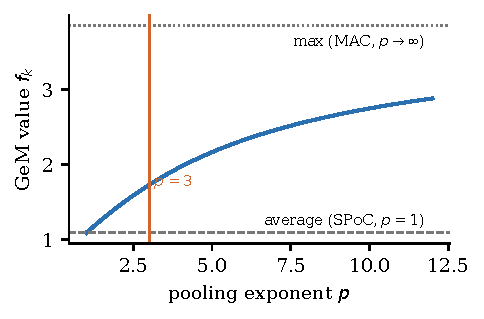
\includegraphics[width=0.55\linewidth]{figures/gem_p.pdf}
\caption{Illustration of GeM pooling (Eq.~\ref{eq:gem}) on a synthetic set of
64 non-negative activations: the pooled value moves continuously from the
average ($p=1$) towards the maximum ($p\rightarrow\infty$). Larger $p$ focuses
the descriptor on the strongest local responses.}
\label{fig:gemp}
\end{figure}

\paragraph{Contrastive loss with SfM tuples.}
Training uses tuples $(q, p, n_1,\dots,n_M)$ with one positive and $M$ hard
negatives. For descriptors $\mathbf{x}_q$ and $\mathbf{x}_j$ and
$d_j=\|\mathbf{x}_q-\mathbf{x}_j\|_2$, the loss is
\begin{equation}
\mathcal{L}= \tfrac12\, d_p^{2} \;+\; \sum_{m=1}^{M}\tfrac12\max\bigl(0,\tau-d_{n_m}\bigr)^{2},
\label{eq:contrastive}
\end{equation}
with margin $\tau$ ($0.85$ for deep backbones \cite{radenovic2019gem}).
Positives are image pairs that share enough 3D points in an SfM model; hard
negatives are the nearest images in descriptor space that belong to a
\emph{different} 3D model, at most one per model, re-mined every epoch.

\paragraph{Learned whitening ($L_w$).}
After training, a linear projection is learned from the descriptors of
matching pairs $(i,j)\in\mathcal{P}$ mined from the SfM models
\cite{radenovic2019gem}. Let
$C_S=\frac{1}{|\mathcal{P}|}\sum_{(i,j)\in\mathcal{P}}(\mathbf{x}_i-\mathbf{x}_j)(\mathbf{x}_i-\mathbf{x}_j)^\top$
be the intra-class covariance, $\boldsymbol\mu$ the mean descriptor and $C_D$
the covariance of non-matching pairs. The whitening is
\begin{equation}
P=\operatorname{eig}\bigl(C_S^{-1/2}\,C_D\,C_S^{-1/2}\bigr)^{\!\top}\,C_S^{-1/2},
\qquad
\mathbf{x}\mapsto\ell_2\bigl(P(\mathbf{x}-\boldsymbol\mu)\bigr),
\label{eq:lw}
\end{equation}
where $\operatorname{eig}(\cdot)$ stacks eigenvectors in decreasing order of
eigenvalue. As in the public implementation, $C_D$ is estimated from the
covariance of all training descriptors.

\paragraph{$\alpha$-weighted query expansion.}
\aqe{} \cite{radenovic2019gem} replaces the query by a weighted sum of itself
and its top-$n$ neighbours,
\begin{equation}
\mathbf{x}_q' = \ell_2\Bigl(\mathbf{x}_q + \sum_{i=1}^{n} \bigl(\mathbf{x}_q^\top\mathbf{x}_{(i)}\bigr)^{\alpha}\,\mathbf{x}_{(i)}\Bigr),
\label{eq:aqe}
\end{equation}
and searches again. Average query expansion \cite{chum2007totalrecall} is the
special case $\alpha=0$.

\subsection{B0: Rebuilding GeM on a Self-Supervised ViT}
\label{sec:b0}

B0 keeps the complete GeM recipe and swaps only the backbone, from ResNet-101
\cite{he2016resnet} to DINOv2 ViT-B/14 \cite{oquab2024dinov2}. An input image,
resized so that its longer side is at most 518 pixels and cropped to a
multiple of the patch size 14, yields one class token
$\mathbf{t}_{\text{cls}}\in\mathbb{R}^{768}$ and an $h\times w$ grid of patch
tokens after the final LayerNorm. We reshape the patch tokens into a
$768\times h\times w$ map and apply
\begin{equation}
\mathbf{x}_{\text{GeM}}=\ell_2\Bigl(\text{GeM}_p\bigl(\text{ReLU}(\mathbf{T}_{\text{patch}})\bigr)\Bigr),
\end{equation}
where the ReLU is required because LayerNorm outputs are signed while
Eq.~\eqref{eq:gem} assumes non-negative inputs. To keep the strong pretrained
representation and fit a free GPU, only the last $B$ of the 12 transformer
blocks (plus the final LayerNorm and $p$) are trained; the first $12-B$
blocks run without gradient. With $B=2$, about 14.2M of the 86M backbone
parameters are trainable. Figure~\ref{fig:pipeline} summarises the pipeline.

Alongside the trained head, the network always exports two diagnostic
descriptors from the same forward pass: the class token
$\mathbf{x}_{\text{CLS}}=\ell_2(\mathbf{t}_{\text{cls}})$ and plain average
pooling of patch tokens without ReLU, $\mathbf{x}_{\text{Avg}}$. They are
evaluated with exactly the same whitening and protocol, which lets the data
tell us which head to train next.

\begin{figure}[t]
\centering
\resizebox{\linewidth}{!}{%
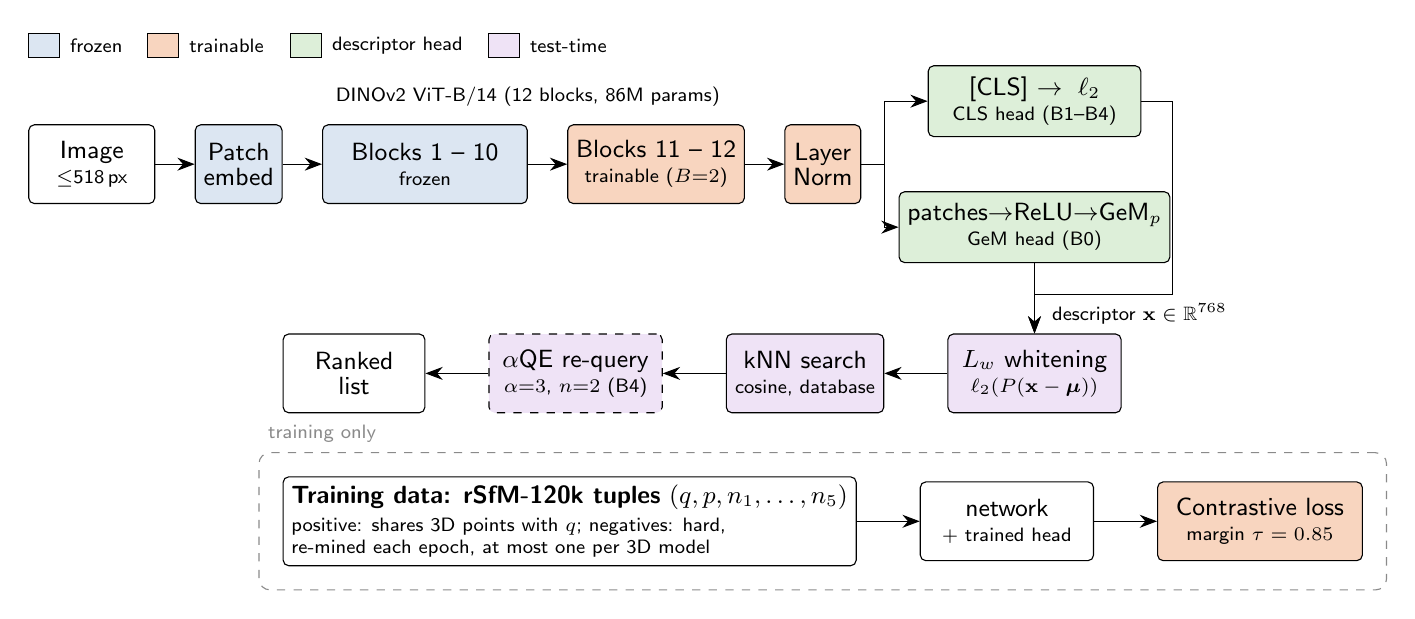
\begin{tikzpicture}[
  font=\sffamily\small, >={Stealth[length=2.2mm]}, node distance=5mm,
  box/.style={draw, rounded corners=2pt, minimum height=10mm, align=center, inner sep=3pt},
  lab/.style={font=\sffamily\scriptsize, align=center},
  sw/.style={draw, minimum width=4mm, minimum height=3mm, inner sep=0pt}]
% ---------------- row 1: backbone ----------------
\node[box, minimum width=16mm] (img) at (0,0) {Image\\[-2pt]\scriptsize $\le$518\,px};
\node[box, fill=cfrozen, right=of img] (pe) {Patch\\[-2pt]embed};
\node[box, fill=cfrozen, right=of pe, minimum width=26mm] (fz) {Blocks 1 -- 10\\[-2pt]\scriptsize frozen};
\node[box, fill=ctrain, right=of fz, minimum width=20mm] (tr) {Blocks 11 -- 12\\[-2pt]\scriptsize trainable ($B{=}2$)};
\node[box, fill=ctrain, right=of tr] (ln) {Layer\\[-2pt]Norm};
\node[lab, above=1mm of fz.north east] {DINOv2 ViT-B/14 (12 blocks, 86M params)};
\draw[->] (img) -- (pe); \draw[->] (pe) -- (fz); \draw[->] (fz) -- (tr); \draw[->] (tr) -- (ln);
% heads
\node[box, fill=chead, minimum width=27mm, minimum height=9mm] (hcls) at ($(ln.east)+(22mm,8mm)$) {[CLS] $\rightarrow\ \ell_2$\\[-2pt]\scriptsize CLS head (B1--B4)};
\node[box, fill=chead, minimum width=27mm, minimum height=9mm] (hgem) at ($(ln.east)+(22mm,-8mm)$) {patches$\rightarrow$ReLU$\rightarrow$GeM$_p$\\[-2pt]\scriptsize GeM head (B0)};
\draw[->] (ln.east) -- ++(3mm,0) |- (hcls.west);
\draw[->] (ln.east) -- ++(3mm,0) |- (hgem.west);
% ---------------- row 2: search (right to left) ----------------
\node[box, fill=cpost, minimum width=22mm] (lw) at ($(hgem.south)+(0,-14mm)$) {$L_w$ whitening\\[-2pt]\scriptsize $\ell_2(P(\mathbf{x}-\boldsymbol\mu))$};
\node[box, fill=cpost, left=8mm of lw, minimum width=20mm] (knn) {kNN search\\[-2pt]\scriptsize cosine, database};
\node[box, fill=cpost, dashed, left=8mm of knn, minimum width=22mm] (qe) {$\alpha$QE re-query\\[-2pt]\scriptsize $\alpha{=}3$, $n{=}2$ (B4)};
\node[box, left=8mm of qe, minimum width=18mm] (rank) {Ranked\\[-2pt]list};
\draw[->] (hcls.east) -- ++(4mm,0) |- ($(lw.north)+(0,5mm)$) -- (lw.north);
\draw[->] (hgem.south) -- ($(lw.north)+(0,5mm)$) -- (lw.north);
\draw[->] (lw) -- (knn); \draw[->] (knn) -- (qe); \draw[->] (qe) -- (rank);
\node[lab, anchor=west] at ($(lw.north)+(1mm,2.5mm)$) {descriptor $\mathbf{x}\in\mathbb{R}^{768}$};
% ---------------- row 3: training ----------------
\node[box, fill=white, minimum width=58mm, align=left, anchor=north west] (tup) at ($(rank.south west)+(0,-8mm)$)
  {\textbf{Training data: rSfM-120k tuples} $(q,p,n_1,\dots,n_5)$\\[-1pt]\scriptsize positive: shares 3D points with $q$; negatives: hard,\\[-3pt]\scriptsize re-mined each epoch, at most one per 3D model};
\node[box, fill=white, right=8mm of tup, minimum width=22mm] (net) {network\\[-2pt]\scriptsize + trained head};
\node[box, fill=ctrain, right=8mm of net, minimum width=26mm] (loss) {Contrastive loss\\[-2pt]\scriptsize margin $\tau=0.85$};
\draw[->] (tup) -- (net); \draw[->] (net) -- (loss);
\begin{scope}[on background layer]
\node[draw=cgray, dashed, rounded corners=4pt, fit=(tup)(net)(loss), inner sep=3mm, label={[lab, text=cgray, anchor=south west]north west:training only}] {};
\end{scope}
% legend
\node[sw, fill=cfrozen, label={[lab]right:frozen}] (l1) at ($(img.north west)+(2mm,10mm)$) {};
\node[sw, fill=ctrain, label={[lab]right:trainable}, right=11mm of l1] (l2) {};
\node[sw, fill=chead, label={[lab]right:descriptor head}, right=14mm of l2] (l3) {};
\node[sw, fill=cpost, label={[lab]right:test-time}, right=21mm of l3] (l4) {};
\end{tikzpicture}}
\caption{Overview of the retrieval pipeline. DINOv2 ViT-B/14 tokens feed two
descriptor heads: GeM over ReLU-rectified patch tokens (the original GeM
design, trained in B0) and the $\ell_2$-normalised class token (trained from
B1 on). The descriptor is whitened with $L_w$, searched with cosine kNN and
optionally expanded with \aqe{} (B4). The dashed
box shows training: the contrastive loss on SfM tuples updates only the last
$B$ blocks, the final LayerNorm and $p$ (orange). In B0 the loss is attached to
the GeM head, in B1--B4 to the CLS head.}
\label{fig:pipeline}
\end{figure}

\subsection{One-Factor-at-a-Time Improvement Protocol}
\label{sec:protocol}

Small benchmarks such as \roxf{} (70 queries) make it easy to over-interpret
differences when several factors change at once. We therefore adopt three
rules. (i) Each version changes \emph{one} factor relative to the best version
so far and keeps everything else, including the random seed. (ii) Before
running, each version records \emph{why} the change is expected to help: the
previous result, the underlying theory, and a supporting paper. (iii) Versions
are compared on a held-out \emph{validation} task built from the rSfM-120k
validation split (Section~\ref{sec:setup}); \roxf{} and \rpar{} are used only
to report results. Differences smaller than about 1 validation mAP, which is
within what a single seed can resolve, are treated as ties, and ties are kept
in the lineage rather than resolved on the test sets. Test-time-only factors
(such as \aqe{}) do not require retraining; they are computed from the stored
descriptors and reported as their own version, with and without the factor.
Fig.~\ref{fig:lineage} shows the resulting lineage.

In the first version of this study the branching decisions were taken on
\roxs{} Medium mAP. We re-ran the selection on validation afterwards with the
saved checkpoints (Table~\ref{tab:val}). It confirms the two decisions that
matter, B0$\rightarrow$B1 (train the class token) and adding \aqe{}, but ranks
B2 slightly above B1 and B3 (93.56 vs.\ 93.13 and 92.73 validation mAP). Since
B1, B2 and B3 lie within 0.8 validation mAP and 0.5 test mAP of each other, we
report them as equivalent and keep B3 as the base of B4, as in the original
lineage; B2 + \aqe{} is reported alongside it.

\begin{figure}[t]
\centering
\resizebox{\linewidth}{!}{%
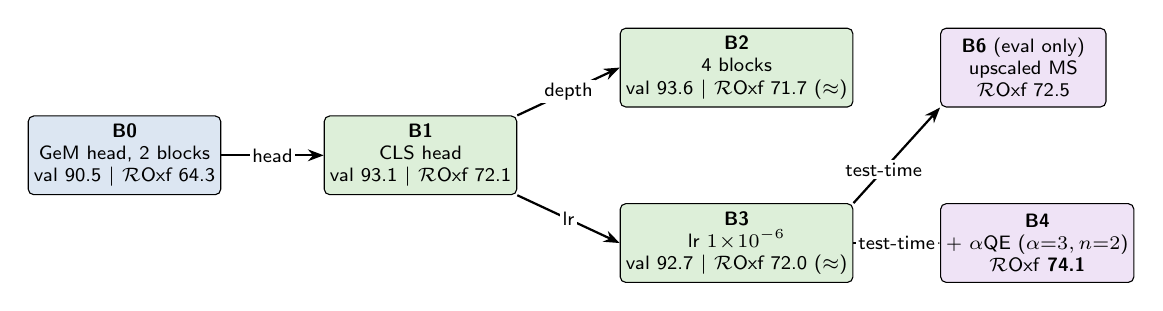
\begin{tikzpicture}[font=\sffamily\scriptsize, >={Stealth[length=2mm]},
  v/.style={draw, rounded corners=2pt, align=center, minimum width=21mm, minimum height=10mm, inner sep=2pt},
  e/.style={->, thick}, el/.style={midway, fill=white, inner sep=1pt, align=center}]
\node[v, fill=cfrozen] (b0) {\textbf{B0}\\GeM head, 2 blocks\\val 90.5 $\mid$ \roxs{} 64.3};
\node[v, fill=chead, right=13mm of b0] (b1) {\textbf{B1}\\CLS head\\val 93.1 $\mid$ \roxs{} 72.1};
\node[v, fill=chead, above right=1mm and 13mm of b1] (b2) {\textbf{B2}\\4 blocks\\val 93.6 $\mid$ \roxs{} 71.7 ($\approx$)};
\node[v, fill=chead, below right=1mm and 13mm of b1] (b3) {\textbf{B3}\\lr $1\!\times\!10^{-6}$\\val 92.7 $\mid$ \roxs{} 72.0 ($\approx$)};
\node[v, fill=cpost, right=11mm of b3] (b4) {\textbf{B4}\\+ \aqe{} ($\alpha{=}3,n{=}2$)\\\roxs{} \textbf{74.1}};
\node[v, fill=cpost, right=11mm of b2] (b6) {\textbf{B6} (eval only)\\upscaled MS\\\roxs{} 72.5};
\draw[e] (b0) -- node[el]{head} (b1);
\draw[e] (b1.north east) -- node[el]{depth} (b2.west);
\draw[e] (b1.south east) -- node[el]{lr} (b3.west);
\draw[e] (b3) -- node[el]{test-time} (b4);
\draw[e] (b3.north east) -- node[el, pos=0.35]{test-time} (b6.south west);
\end{tikzpicture}}
\caption{Experimental lineage. Each arrow changes exactly one factor. ``val''
is the rSfM-120k validation mAP used for selection, \roxs{} the Medium mAP
reported on the test set (trained head, single scale, $L_w$; B6: multi-scale
with $L_w$). B1, B2 and B3 are within the tie margin ($\approx$). B6 is an
evaluation-only check on the B3 checkpoint; the planned ViT-L/14 version (B5)
was not run.}
\label{fig:lineage}
\end{figure}

The versions and their motivation are:
\begin{description}
\item[B1 -- train the CLS head instead of GeM.] In B0 the untrained class
token of the fine-tuned network outperformed the trained GeM head by
+5.0/+4.0 mAP (\roxs{} M/H, single scale, $L_w$), and DINOv2 itself uses the
class token for retrieval \cite{oquab2024dinov2,elnouby2021vitretrieval}.
\item[B2 -- fine-tune 4 blocks instead of 2.] Two of twelve blocks may lack
the capacity to adapt to landmarks \cite{elnouby2021vitretrieval}.
\item[B3 -- learning rate $2\times10^{-6}\rightarrow1\times10^{-6}$ (from B1).]
B2 lowered the training loss but not test accuracy, suggesting the features
drift away from the pretrained solution; a smaller step keeps the model closer
to it \cite{kumar2022distort}, and \cite{radenovic2019gem} also used very small
learning rates.
\item[B4 -- add \aqe{} at test time (on B3).] A cheap, training-free
post-processing that is known to help on Oxford/Paris \cite{radenovic2019gem}.
\item[B6 -- up-scaled multi-scale inference (on B3, evaluation only).] B0 and
B1 showed that the default scales $\{1,1/\sqrt2,1/2\}$ lower the class token
(Section~\ref{sec:heads}); if the cause is the loss of resolution at small
scales, replacing them with $\{\sqrt2,1,1/\sqrt2\}$ should remove the drop.
\end{description}

% =====================================================================
\section{Experimental Setup}
\label{sec:setup}

\paragraph{Training data.}
We train on retrieval-SfM-120k \cite{radenovic2016cnn,radenovic2019gem}, built
from 3D models reconstructed from Flickr photos \cite{schonberger2015sfm}. The
training split contains 551 models (about 133k images) and the validation
split 162 models; models overlapping with the Oxford and Paris test landmarks
were removed by the dataset authors. No manual labels are used.

\paragraph{Validation task.}
For model selection we build a retrieval task from the validation split: 1,000
query images and a database of 5,000 images drawn from the 162 validation
models (fixed seed), where a database image is relevant if it belongs to the
same 3D model as the query (on average 41.2 relevant images per query). We
report validation mAP and mP@10 of each model's trained head with $L_w$, and
tune the \aqe{} parameters on a grid $\alpha\in\{0,1,3,5,10\}$,
$n\in\{1,2,3,5,10\}$ on the same task.

\paragraph{Test data and metrics.}
We evaluate on \roxf{} and \rpar{} \cite{radenovic2018revisiting}
(4,993 and 6,322 database images, 70 queries each), the revisited versions of
Oxford5k \cite{philbin2007oxford} and Paris6k \cite{philbin2008paris}. Queries
are cropped to their bounding box. We report mean average precision (mAP) under
the Easy (E), Medium (M) and Hard (H) protocols, and mean precision at 10
(mP@10) where available. The 1M distractor set is not used.

\paragraph{Implementation details.}
All models use the DINOv2 ViT-B/14 weights from the official repository
\cite{oquab2024dinov2} and are implemented in PyTorch \cite{paszke2019pytorch}.
Table~\ref{tab:hparams} lists the hyper-parameters, which follow the original
GeM recipe wherever possible. Each epoch re-mines hard negatives for 2,000
random queries from a pool of 22,000 images, with 5 negatives per tuple;
gradients are accumulated over 5 tuples per optimizer step. Training uses
Adam \cite{kingma2015adam} with exponential learning-rate decay
($\gamma=e^{-0.01}$ per epoch), weight decay $10^{-6}$, a $10\times$ larger
learning rate for $p$, and fp16 mixed precision. $L_w$ is learned on 5,000
matching pairs from the rSfM-120k whitening split. Multi-scale (MS)
descriptors average the descriptors at scales $\{1, 1/\sqrt2, 1/2\}$ (GeM-style
power mean for the GeM head, arithmetic mean for the signed CLS/Avg
descriptors); single scale (SS) uses scale 1 only. The frozen DINOv2 baseline
is evaluated with exactly the same code, resolution, $L_w$ (learned on its own
descriptors) and \aqe{}. Every run uses seed 0 and
one NVIDIA T4 GPU (16\,GB) on Kaggle; one epoch takes about 21 minutes with 2
trainable blocks and 23.5 minutes with 4, and a complete run (data download,
10 epochs, whitening and evaluation) takes 4.5--5 hours.

\begin{table}[t]
\centering
\caption{Training and evaluation settings. Only the highlighted factor changes
between consecutive versions.}
\label{tab:hparams}
\setlength{\tabcolsep}{4pt}
\begin{adjustbox}{max width=\textwidth}
\begin{tabular}{@{}lcccccc@{}}
\toprule
 & Frozen & B0 & B1 & B2 & B3 & B4 \\
\midrule
Trained head          & -- & GeM & \textbf{CLS} & CLS & CLS & CLS \\
Fine-tuned blocks     & 0 & 2 & 2 & \textbf{4} & 2 & 2 \\
Learning rate         & -- & $2\!\times\!10^{-6}$ & $2\!\times\!10^{-6}$ & $2\!\times\!10^{-6}$ & $\mathbf{1\!\times\!10^{-6}}$ & $1\!\times\!10^{-6}$ \\
Query expansion       & -- & -- & -- & -- & -- & \textbf{\aqe{}} \\
\bottomrule
\end{tabular}
\end{adjustbox}\\[3pt]
\parbox{0.92\linewidth}{\footnotesize\emph{Shared by all versions:} DINOv2
ViT-B/14; rSfM-120k; contrastive loss, $\tau=0.85$; 10 epochs; 518\,px
(train/test); GeM $p_0=3$; Adam, weight decay $10^{-6}$; $L_w$ from 5k pairs;
\aqe{} with $\alpha=3$, $n=2$; seed 0.}
\end{table}

% =====================================================================
\section{Results}
\label{sec:results}

\subsection{Main Results}

Table~\ref{tab:main} reports every version with its trained descriptor, single
scale and learned whitening, the frozen DINOv2 backbone evaluated under our
protocol, and reference numbers taken from the literature.
Figure~\ref{fig:progression} visualises the same numbers, and
Table~\ref{tab:val} gives the validation scores used for selection.

\begin{table}[t]
\centering
\caption{Main results (mAP, \%) on the revisited benchmarks. Our rows use
single-scale descriptors with $L_w$; $\Delta$ is the change in \roxs{} Medium
w.r.t.\ the version each row branches from; ``val'' is the rSfM-120k
validation mAP. Rows with and without \aqe{} are grouped so that each is
compared with its counterpart. Reference rows are copied from the cited
sources and differ in protocol (\dag: multi-scale with whitening, from the
official cnnimageretrieval-pytorch release of \cite{radenovic2019gem};
\ddag: frozen backbone, Table~9 of \cite{oquab2024dinov2}).}
\label{tab:main}
\setlength{\tabcolsep}{4pt}
\begin{adjustbox}{max width=\textwidth}
\begin{tabular}{@{}llcccccccc@{}}
\toprule
 & & & \multicolumn{3}{c}{\roxf} & \multicolumn{3}{c}{\rpar} & \\
\cmidrule(lr){4-6}\cmidrule(lr){7-9}
Version & Descriptor & val & E & M & H & E & M & H & $\Delta$M \\
\midrule
\multicolumn{10}{@{}l}{\emph{Reference results (other protocols)}}\\
GeM R101\dag{} \cite{radenovic2019gem} & GeM & -- & -- & 65.4 & 40.1 & -- & 76.7 & 55.2 & \\
DINOv2 ViT-B/14\ddag{} \cite{oquab2024dinov2} & CLS & -- & -- & 72.9 & 49.5 & -- & 90.3 & 78.6 & \\
\midrule
\multicolumn{10}{@{}l}{\emph{Ours, no query expansion (DINOv2 ViT-B/14, global descriptor only)}}\\
Frozen DINOv2 & CLS & 90.96 & 85.15 & 70.06 & 49.84 & 94.24 & 88.64 & 75.96 & -- \\
B0 & GeM (trained) & 90.50 & 77.71 & 64.30 & 44.17 & 93.05 & 85.87 & 71.60 & -- \\
B0 & CLS (not trained) & 91.13 & 83.76 & 69.28 & 48.19 & 93.76 & 88.30 & 74.73 & \\
B1: CLS head & CLS & 93.13 & \best{85.71} & \best{72.10} & \best{52.88} & 95.53 & 89.72 & 76.46 & +7.80 \\
B2: 4 blocks & CLS & \best{93.56} & 85.01 & 71.67 & 52.77 & 95.21 & 89.70 & 76.04 & $-$0.43 \\
B3: lr $10^{-6}$ & CLS & 92.73 & 85.64 & 71.99 & 52.77 & 95.17 & \best{89.83} & \best{77.06} & $-$0.11 \\
\midrule
\multicolumn{10}{@{}l}{\emph{Ours, with \aqe{} ($\alpha=3$, $n=2$)}}\\
Frozen DINOv2 + \aqe & CLS & -- & 87.33 & 72.17 & 51.85 & 94.45 & 89.06 & 76.62 & -- \\
B2 + \aqe & CLS & -- & 87.06 & 73.61 & \best{54.68} & 95.30 & 89.88 & 76.31 & +1.94 \\
B4: B3 + \aqe & CLS & -- & \best{87.91} & \best{74.09} & 54.60 & \best{95.58} & \best{90.17} & \best{77.73} & +2.10 \\
\bottomrule
\end{tabular}
\end{adjustbox}
\end{table}

\begin{figure}[t]
\centering
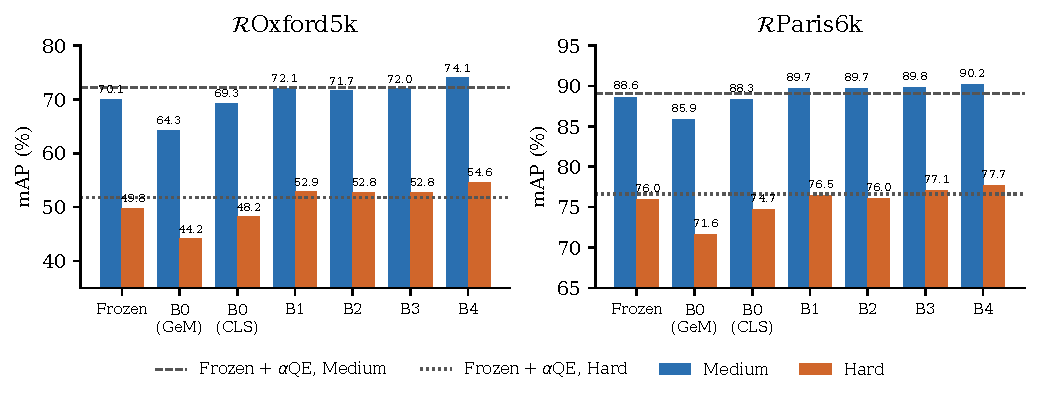
\includegraphics[width=\linewidth]{figures/progression.pdf}
\caption{mAP across versions (single scale, $L_w$), including the frozen
DINOv2 backbone under our protocol. Dashed and dotted lines are the frozen
backbone \emph{with} \aqe{}, the fair counterpart of B4. All fine-tuned
class-token models (B1--B3) are on par with it on \roxf{} Medium and above it
on Hard without any query expansion.}
\label{fig:progression}
\end{figure}

Four observations stand out. First, simply replacing ResNet-101 by DINOv2
ViT-B/14 in the GeM recipe (B0, GeM head) already improves \rpar{} strongly
(85.9/71.6 vs.\ 76.7/55.2) and \roxf{} Hard (44.2 vs.\ 40.1), but \roxf{}
Medium stays at the ResNet level. Second, switching the trained descriptor
from GeM to the class token (B1) is the largest single improvement:
+7.8/+8.7 mAP on \roxf{} M/H over the B0 GeM head and +2.8/+4.7 over the
untrained B0 class token, which shows that the gain comes both from the choice
of descriptor and from training it directly. Third, B2 and B3 do not move the
\roxf{} Medium score beyond the $\pm0.5$ range around 72; only test-time
\aqe{} (B4) adds a further +2.1/+1.8 on \roxf{} and +0.3/+0.7 on \rpar{}.
Fourth, the comparison with the frozen backbone must be made under the same
protocol. Evaluated with our code, the frozen DINOv2 class token with $L_w$
reaches 70.1/49.8 on \roxf{} and 88.6/76.0 on \rpar{}. Fine-tuning therefore
helps, but by a moderate margin: +1.9/+2.9 (B3) on \roxf{} and +1.2/+1.1 on
\rpar{} without query expansion, and +1.9/+2.8 and +1.1/+1.1 when \aqe{} is
applied to both. Note that B0, which fine-tunes through the GeM head, is
\emph{below} the frozen class token; the benefit of fine-tuning appears only
once the class token itself is trained. The published DINOv2 figures
\cite{oquab2024dinov2} (72.9/49.5 and 90.3/78.6) were obtained with a
different evaluation protocol and are listed for reference only.

\begin{table}[t]
\centering
\caption{Selection on the rSfM-120k validation task (1,000 queries, 5,000
database images; trained head, single scale). Loss: contrastive loss of the
trained head on validation tuples. Bold: best.}
\label{tab:val}
\setlength{\tabcolsep}{4pt}
\begin{adjustbox}{max width=\textwidth}
\begin{tabular}{@{}lcccccc@{}}
\toprule
 & Frozen & B0 (GeM) & B0 (CLS) & B1 & B2 & B3 \\
\midrule
val mAP          & 87.81 & 88.11 & 88.62 & 91.41 & \best{91.62} & 90.61 \\
val mAP + $L_w$  & 90.96 & 90.50 & 91.13 & 93.13 & \best{93.56} & 92.73 \\
val mP@10 + $L_w$ & 98.10 & 98.20 & 98.55 & 98.89 & \best{99.06} & 98.83 \\
val loss         & 0.142 & 0.109 & 0.113 & 0.092 & \best{0.081} & 0.098 \\
\bottomrule
\end{tabular}
\end{adjustbox}
\end{table}

The validation task (Table~\ref{tab:val}) agrees with the test sets on the
large effects: training the class token (B1) gains +2.6 validation mAP over
the B0 GeM head and +2.2 over the frozen backbone. It ranks B2 first, but the
spread among B1--B3 (0.8 mAP) is of the same size as their spread on the test
sets (0.4 mAP on \roxs{} Medium), and the two orderings differ, so we do not
read a winner into it. Validation-selected B2 with \aqe{} gives 73.6/54.7 on
\roxf{} and 89.9/76.3 on \rpar{}, within 0.5 mAP of B4.

\subsection{Descriptor Head, Whitening and Scale}
\label{sec:heads}

Table~\ref{tab:heads} and Fig.~\ref{fig:heads} break down all descriptor
variants exported by B0 and B1. Learned whitening consistently helps on
\roxf{} (e.g.\ +4.7 mAP Medium for the B0 class token), while its effect on
\rpar{} is small. In B0, multi-scale averaging gives the usual small gain to
the GeM head (+0.9 M) but already reduces the class token (69.3$\rightarrow$68.5).
Once the class token is trained (B1), multi-scale hurts it by 2.3 mAP Medium;
we therefore use single scale for all CLS results. The B6 check
(Table~\ref{tab:ablation}, bottom) shows that the drop comes from the
down-scaled inputs and not from averaging itself: on the B3 checkpoint,
replacing $\{1,1/\sqrt2,1/2\}$ by $\{\sqrt2,1,1/\sqrt2\}$ turns a $-$2.1 mAP loss
into a +0.5 gain on \roxs{} Medium (72.5 vs.\ 72.0; 75.1 vs.\ 74.1 with \aqe{}),
while \rpar{} is unchanged. The gain is small and comes at about twice the
extraction cost, so single scale remains our default. Finally, in B1 the GeM and
Avg heads, which are no longer trained, collapse (to about 55 M / 30 H on
\roxf{} with $L_w$), confirming that the last blocks have specialised to the
class-token objective.

\begin{table}[t]
\centering
\caption{Descriptor heads of B0 and B1 on \roxf{} / \rpar{} (mAP Medium/Hard).
SS/MS: single/multi-scale; $L_w$: learned whitening. Bold: best per model.}
\label{tab:heads}
\setlength{\tabcolsep}{3.2pt}
\begin{adjustbox}{max width=\textwidth}
\begin{tabular}{@{}llcccc@{\hskip 8pt}cccc@{}}
\toprule
 & & \multicolumn{4}{c}{B0 (GeM head trained)} & \multicolumn{4}{c}{B1 (CLS head trained)}\\
\cmidrule(lr){3-6}\cmidrule(lr){7-10}
Head & Setting & \roxs{} M & H & \rpas{} M & H & \roxs{} M & H & \rpas{} M & H \\
\midrule
\multirow{4}{*}{GeM}
 & SS        & 61.27 & 43.03 & 86.09 & 71.99 & 37.26 & 12.07 & 71.63 & 48.97 \\
 & SS + $L_w$ & 64.30 & 44.17 & 85.87 & 71.60 & 55.85 & 30.47 & 83.34 & 67.27 \\
 & MS        & 62.58 & 44.35 & 86.43 & 72.66 & 39.57 & 14.29 & 74.97 & 53.84 \\
 & MS + $L_w$ & 65.15 & 45.31 & 87.21 & 73.33 & 55.71 & 29.74 & 83.70 & 67.87 \\
\midrule
\multirow{4}{*}{CLS}
 & SS        & 64.59 & 45.21 & 87.33 & 73.49 & 70.41 & 50.51 & 88.99 & 75.74 \\
 & SS + $L_w$ & \best{69.28} & 48.19 & 88.30 & 74.73 & \best{72.10} & \best{52.88} & \best{89.72} & \best{76.46} \\
 & MS        & 65.41 & 48.22 & 87.69 & 74.22 & 67.79 & 47.19 & 88.74 & 75.45 \\
 & MS + $L_w$ & 68.45 & \best{48.98} & \best{88.63} & \best{75.45} & 69.82 & 50.77 & 89.53 & 76.36 \\
\midrule
\multirow{4}{*}{Avg}
 & SS        & 62.08 & 44.55 & 85.62 & 71.47 & 36.18 & 11.99 & 71.98 & 50.21 \\
 & SS + $L_w$ & 65.81 & 45.60 & 86.86 & 73.16 & 54.14 & 26.71 & 82.91 & 66.85 \\
 & MS        & 62.54 & 45.04 & 86.07 & 72.13 & 38.33 & 14.22 & 75.23 & 55.14 \\
 & MS + $L_w$ & 64.86 & 45.51 & 87.26 & 73.68 & 53.81 & 26.42 & 83.10 & 67.41 \\
\bottomrule
\end{tabular}
\end{adjustbox}
\end{table}

\begin{figure}[t]
\centering
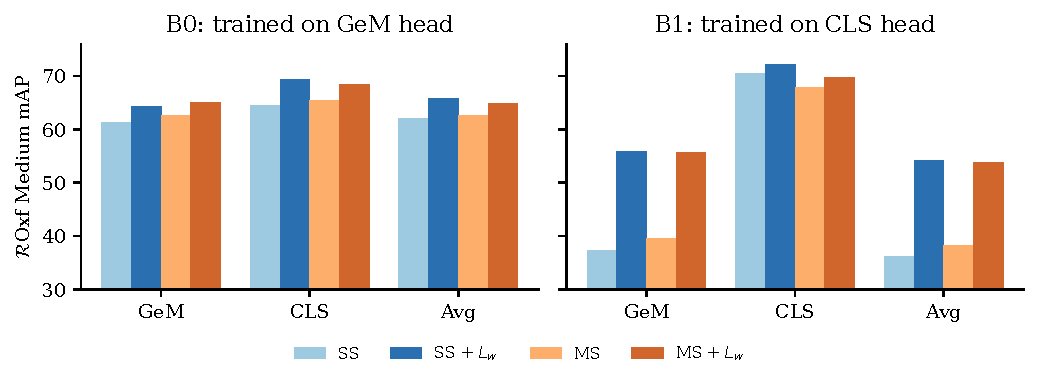
\includegraphics[width=\linewidth]{figures/heads_ablation.pdf}
\caption{\roxs{} Medium mAP of the three descriptor heads under four test
settings. Left: B0, trained through the GeM head; right: B1, trained through
the class token. Training the class token improves it and makes the other two
heads collapse; multi-scale averaging lowers the class token in both models.}
\label{fig:heads}
\end{figure}

\begin{table}[t]
\centering
\caption{Evaluation-only checks (mAP Medium/Hard, $L_w$). Top: pooling variants
on the B0 checkpoint (trained through standard GeM), single scale. GeM-signed
removes the ReLU and applies a signed power mean; GeM-shift subtracts the
per-channel minimum before GeM. Bottom: multi-scale variants on the B3
checkpoint (class token).}
\label{tab:ablation}
\setlength{\tabcolsep}{4pt}
\begin{adjustbox}{max width=\textwidth}
\begin{tabular}{@{}llcccccc@{}}
\toprule
 & & \multicolumn{2}{c}{\roxs{} (no QE)} & \multicolumn{2}{c}{\rpas{} (no QE)} & \multicolumn{2}{c}{\roxs{} + \aqe{}}\\
\cmidrule(lr){3-4}\cmidrule(lr){5-6}\cmidrule(lr){7-8}
Model & Variant & M & H & M & H & M & H \\
\midrule
B0 & GeM (ReLU, trained) & 64.31 & 44.20 & 85.87 & 71.60 & -- & -- \\
B0 & GeM-signed (no ReLU) & 64.86 & 45.00 & 86.90 & 73.10 & -- & -- \\
B0 & GeM-shift ($x-\min$) & 52.90 & 33.81 & 79.49 & 62.49 & -- & -- \\
B0 & Avg (no ReLU) & 65.81 & 45.60 & 86.86 & 73.17 & -- & -- \\
B0 & CLS (not trained) & \best{69.29} & \best{48.19} & \best{88.30} & \best{74.74} & -- & -- \\
\midrule
B3 & SS: $\{1\}$ & 71.99 & 52.77 & 89.83 & 77.06 & 74.09 & 54.60 \\
B3 & MS: $\{1,1/\sqrt2,1/2\}$ & 69.88 & 50.44 & 89.57 & 76.72 & 72.49 & 53.58 \\
B3 & B6, MS-up: $\{\sqrt2,1,1/\sqrt2\}$ & \best{72.49} & \best{53.57} & 89.80 & \best{77.12} & \best{75.09} & \best{55.44} \\
\bottomrule
\end{tabular}
\end{adjustbox}
\end{table}

\subsection{Fine-Tuning Depth and Learning Rate}

Figure~\ref{fig:loss} plots the training loss of B1--B3. Fine-tuning four
blocks (B2) lowers the final contrastive loss by 24\% (0.076 vs.\ 0.099) and
also gives the best validation loss and mAP (Table~\ref{tab:val}), yet yields
slightly \emph{lower} test accuracy on both datasets (Table~\ref{tab:main}).
Halving the learning rate (B3) leaves a higher final loss (0.116), a lower
validation mAP and the same \roxf{} accuracy (72.0/52.8), with a small gain on
\rpar{} Hard (+0.6). Training and validation, which come from the same SfM
distribution, move together, but the test benchmarks do not follow: after B1,
better fitting rSfM-120k no longer transfers to Oxford and Paris.

\begin{figure}[t]
\centering
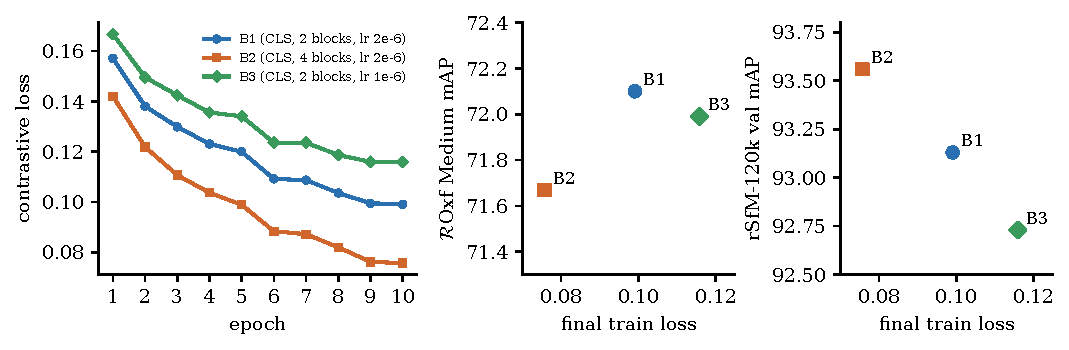
\includegraphics[width=\linewidth]{figures/train_loss.pdf}
\caption{Left: training loss per epoch for B1--B3 (from the training logs).
Middle: final training loss versus \roxs{} Medium mAP. Right: final training
loss versus rSfM-120k validation mAP. B2 fits the training data best and is
best on validation, but retrieves slightly worse on the test set.}
\label{fig:loss}
\end{figure}

\subsection{Query Expansion}

Table~\ref{tab:qe} isolates the effect of \aqe{} on the B3 model. With
$\alpha=3$ and $n=2$, \aqe{} improves every metric on \roxf{}, including
precision at 10 (+1.9 M, +3.6 H), and gives smaller but consistent gains on
\rpar{} mAP. The improvement holds for both single- and multi-scale
descriptors, but single scale remains the better choice.

The setting $\alpha=3$, $n=2$ is the one commonly used in the literature
\cite{radenovic2019gem}. Tuning it on the validation task instead selects
$\alpha=0$, $n=10$, i.e.\ plain average query expansion over ten neighbours
(94.71 vs.\ 93.96 validation mAP for B2 with $\alpha=3$, $n=2$; the trend is
the same for the frozen backbone and B3). This choice does not transfer
uniformly (last row of Table~\ref{tab:qe}): it raises \rpar{} to 91.1/79.3 but
lowers \roxf{} to 69.8/50.1, below no expansion at all. The validation task has
about 41 relevant images per query, so expanding with many neighbours is safe
there; \roxf{} has far fewer relevant images per query and many hard negatives,
so large $n$ pulls in false positives. We therefore keep $\alpha=3$, $n=2$ as
the main setting and report the validation choice for transparency; a
validation set whose statistics are closer to the test landmarks would be
needed to tune \aqe{} reliably.

\begin{table}[t]
\centering
\caption{Effect of \aqe{} on the B3 model, CLS descriptor with $L_w$.
B4 = B3 + \aqe{} ($\alpha=3$, $n=2$), single scale. The last row uses the
setting chosen on validation ($\alpha=0$, $n=10$).}
\label{tab:qe}
\setlength{\tabcolsep}{3.5pt}
\begin{adjustbox}{max width=\textwidth}
\begin{tabular}{@{}llcccccccc@{}}
\toprule
 & & \multicolumn{4}{c}{\roxf} & \multicolumn{4}{c}{\rpar}\\
\cmidrule(lr){3-6}\cmidrule(lr){7-10}
Scale & QE & M & H & mP@10 M & mP@10 H & M & H & mP@10 M & mP@10 H\\
\midrule
SS & --    & 71.99 & 52.77 & 86.43 & 66.11 & 89.83 & 77.06 & 98.00 & 89.00\\
SS & \aqe  & \best{74.09} & \best{54.60} & \best{88.29} & \best{69.68} & 90.17 & 77.73 & \best{98.14} & 89.00\\
MS & --    & 69.88 & 50.44 & 84.81 & 61.41 & 89.57 & 76.72 & 98.00 & 88.43\\
MS & \aqe  & 72.49 & 53.58 & 86.29 & 66.41 & 89.89 & 77.24 & 97.86 & 88.14\\
\midrule
SS & \aqe{} (0, 10) & 69.76 & 50.11 & 84.14 & 67.14 & \best{91.09} & \best{79.26} & 98.00 & \best{89.14}\\
\bottomrule
\end{tabular}
\end{adjustbox}
\end{table}

% =====================================================================
\section{Discussion}
\label{sec:discussion}

\paragraph{Why does the class token beat GeM on a ViT?}
GeM was designed for CNN feature maps whose post-ReLU activations are
non-negative and spatially sparse, so that a power mean highlights
discriminative regions. ViT patch tokens after LayerNorm are dense and signed,
so a ReLU has to be inserted before GeM. A natural hypothesis is that this ReLU
throws away useful negative evidence. Our ablation (Table~\ref{tab:ablation},
top) does not support it as the main cause: a signed power mean without ReLU
gains only +0.6/+0.8 mAP on \roxf{} (+1.0/+1.5 on \rpar{}) over standard GeM,
and plain average pooling, which also keeps the sign, behaves the same; both
remain 3.5--5 mAP below the untrained class token. Making the tokens
non-negative by shifting instead of clipping is clearly harmful
($-$11.4 mAP), because the shift is dominated by a few extreme values. The gap
is therefore a property of \emph{what} is pooled rather than of the ReLU: any
uniform pooling over patch tokens, including the few high-norm artefact tokens
that large self-supervised ViTs place in background regions
\cite{darcet2024registers}, mixes in non-discriminative content, whereas the
class token is precisely the output that DINOv2's self-distillation objective
shapes into a global image summary \cite{caron2021dino,oquab2024dinov2}. The
learned GeM exponent in B0 stayed close to its initial value ($p=2.956$),
which also suggests that the GeM head did not find a better operating point on
these tokens. We did not test the artefact-token explanation directly (e.g.\
with register tokens), so it remains a plausible but unverified account.

\paragraph{Why does multi-scale hurt the class token?}
For CNNs, multi-scale averaging adds robustness to object size. A ViT trained
at a fixed resolution sees fewer patches at scales $1/\sqrt2$ and $1/2$ (as
few as $18\times18$ tokens), and its position embeddings must be interpolated;
the class token at small scales therefore summarises a coarser, less
discriminative view, and averaging it with the full-scale token dilutes the
descriptor. The B6 check supports this explanation: with the same averaging
but scales $\{\sqrt2,1,1/\sqrt2\}$, the drop disappears and \roxf{} gains
+0.5/+0.8 mAP over single scale (Table~\ref{tab:ablation}). The scale at
$1/\sqrt2$ is still included in B6, so the result points at the smallest scale
($1/2$) as the main source of the loss.

\paragraph{How much does fine-tuning help?}
Under the same protocol the gain of fine-tuning over the frozen DINOv2 class
token is real but moderate (about +2/+3 mAP on \roxf{} and +1 on \rpar{}),
and it exists only when the class token itself is trained: B0, trained through
GeM, ends below the frozen backbone. The strong frozen baseline is consistent
with DINOv2's design as a general-purpose feature extractor
\cite{oquab2024dinov2}, and it means that, for this backbone, the choice of
descriptor matters more than the amount of fine-tuning.

\paragraph{Saturation of fine-tuning.}
B1--B3 all land within 0.5 mAP of each other on \roxf{} Medium, and the B2
experiment shows that more trainable capacity improves the training and
validation objectives without improving retrieval on the test landmarks. This agrees with the observation that fine-tuning
can distort pretrained features and hurt transfer to a shifted distribution
\cite{kumar2022distort}: rSfM-120k is relatively small and visually different
from the Oxford and Paris landmarks, so beyond a light adaptation the model
starts to specialise to the training set. The remaining levers are therefore a
stronger backbone (e.g.\ ViT-L/14), a larger and more diverse training set such
as GLDv2 \cite{weyand2020gldv2} with margin losses \cite{deng2019arcface}, or
post-processing and re-ranking \cite{iscen2017diffusion,shao2023superglobal}.

\paragraph{Limitations.}
The study is limited by a free GPU budget of roughly 30 hours per week, which
shaped several choices. (i) Each configuration was trained once with seed 0;
we did not measure run-to-run variance, so differences below about 1 mAP
(B1 vs.\ B2 vs.\ B3, on validation or test) should be read as ties, and the
fine-tuning gain over the frozen backbone (about 2 mAP on \roxf{}) should be
confirmed with more seeds. (ii) The branching decisions were originally taken
on \roxf{}; the validation selection was carried out afterwards with the saved
checkpoints and agrees on the large effects but not on the ranking of
B1--B3. (iii) Our validation task has many more relevant images per query
than \roxf{}, which made it unreliable for tuning \aqe{}. (iv) The ViT-L/14
version (B5) was not run, and B6 and the GeM ablations are evaluation-only
checks on existing checkpoints rather than retrained models. (v) We do not
evaluate with the $\mathcal{R}$1M distractors, and we do not compare against
two-stage systems with local-feature re-ranking (e.g.\ CVNet
\cite{lee2022cvnet}) or against SuperGlobal \cite{shao2023superglobal}, which
operate in a different cost regime. The external reference numbers in
Table~\ref{tab:main} use different protocols and are indicative only; our own
frozen-backbone rows are the fair baseline.

% =====================================================================
\section{Conclusion}
\label{sec:conclusion}

We revisited the GeM landmark-retrieval recipe with a self-supervised DINOv2
ViT-B/14 backbone and improved it through a transparent one-factor-at-a-time
protocol, with selection on a validation split and a frozen baseline run
under the same protocol. The study shows that, on a ViT, the class token rather
than GeM pooling of patch tokens is the descriptor worth training, and that the
gap is not caused by the ReLU in GeM; that multi-scale averaging hurts the
class token when it adds down-scaled inputs, but not when it up-scales; and
that once the right descriptor is trained, neither more trainable blocks nor a
smaller learning rate helps. Fine-tuning the class token on rSfM-120k improves
over the frozen DINOv2 backbone by about +2/+3 mAP on \roxf{} and +1 on
\rpar{}. With \aqe{} added at test time, the resulting global-only model
reaches 74.1/54.6 mAP on \roxf{} and 90.2/77.7 on \rpar{}, against 72.2/51.9
and 89.1/76.6 for the frozen backbone with the same \aqe{}. Future work
includes repeated seeds, a larger backbone, training on GLDv2, a validation
set closer to the test landmarks, and efficient global re-ranking.

\paragraph{Code and data availability.}
All notebooks, source code, raw result files and training and evaluation
logs used in this paper (B0--B4, the frozen baseline, the validation selection
and the evaluation-only checks) are included in the accompanying repository.
The fine-tuned weights are available from the authors on request.
The datasets are publicly available from their original authors
\cite{radenovic2019gem,radenovic2018revisiting}.

\begin{credits}
\subsubsection{\ackname}
The authors thank Kaggle for the free GPU quota used in all experiments.

\subsubsection{\discintname}
The authors have no competing interests to declare that are relevant to the
content of this article.
\end{credits}

\bibliographystyle{splncs04}
\bibliography{refs}

\end{document}
